\documentclass{article}
\usepackage[utf8]{inputenc}
\usepackage{graphicx}
\usepackage{hyperref}
\usepackage[margin=1in]{geometry} 
\title{How I develop directional bias from fundamental and sentiment analysis in currency trading}
\date{April 2023}
\begin{document}
\maketitle

\section{My opinion toward Fundamental analysis in equity market}
I'm not Warren Buffett, so I'm not going to say something like, "Technical analysis is like looking in the rearview mirror while driving. Fundamental analysis, on the other hand, is like looking through the windshield," because I think that's a false statement. Technical analysis can also provide a forward-looking perspective too if you change the timeframe to a week or a month. To share with you, I began my investment journey with a book called "Gone Fishing with Buffett" and to be honest, I don't think it's beneficial for my trading journey as it oversimplifies so many concepts. 

\section{My opinion toward Fundamental Analysis in Forex market}
I think that the context of Fundamental Analysis in Forex and Equity is extremely different. In equity trading, everyone wants to make money from the market, so someone with better insight - usually an institutional trader - often comes out on top. Retail traders who buy a stock with strong fundamentals usually do so after the financial report has been released and the P/E ratio has already skyrocketed. While a stock with a solid financial report and a low P/E ratio may seem promising to retail traders, only those with more insider information know why the P/E ratio is low - and once again, those are usually institutional traders. My point is that making accurate fundamental analyses requires too much effort for retail traders.

However, in the Forex market, there is a group of players called "Commercial" who account for almost half of the transactions in some currency pairs. They are not there to make money from the market since it is not their core business. Their primary goal is to stabilize the value of the currency they are holding. Hence, with solid fundamental analysis, we can catch some profitable opportunities from them. 

\section{Sentiment Analysis}
Before I dive into fundamental analysis, another easier analysis that indicates the supply and demand dynamics of the market is sentiment analysis. There are two types of sentiment analysis - retail sentiment and institutional sentiment. The analysis below will explore how the sentiment of these two groups of investors affects the price.

\subsection{Retail Sentiment}
Before we dive into the data analysis part, let's see what folk on the internet think about retail sentiment. \\ \\ 
\textbf{Trader Nick and most youtubers}: 95\% of retail trader is on the wrong side of the market, hence, we should take the opposite position of the retail trader. \\ \\
\textbf{FXEmpire}: Forex is the market where the smartest individual traders see where the “dumb money” goes, so it's best to avoid trading along with it or against it. Because you can never know how the smartest money would exploit the opportunity. \\ \\
\textbf{reddit people}: I lost a lot of money by trying to short at "resistances" and buy at "supports so as retail traders. \\ \\
\textbf{DailyFX}: Publish a regular contrarian index openly stating that its market view on a given pair is diametrically opposed to that of the retail sector. \\ \\
Above are the opinions of people on the internet, it seems everyone tends to agree that we should trade against retail. However, let's explore the data. \\ \\ 

\subsubsection{Validating folk's opinion with data}
\begin{center}
    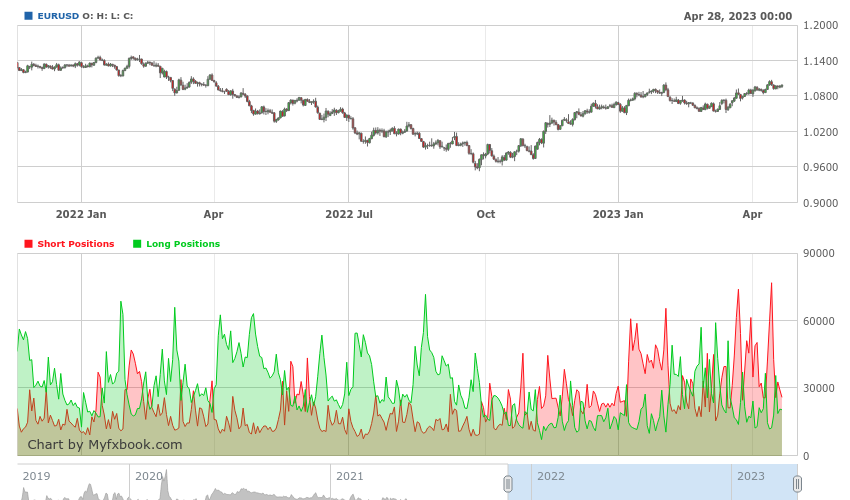
\includegraphics[scale=0.5]{p1.png}    
\end{center}
The screenshot above displays the retail sentiment and the price of EURUSD. It can be observed that when the retail crowd holds long positions, the price tends to decrease, whereas when the retail investors have short positions, the price tends to increase. However, we should validate this observation numerically. Since we cannot access the numerical data directly and only have access to the graph, I will use a computer vision algorithm to convert the graph into numerical data for further analysis. 

%https://www.reddit.com/r/Forex/comments/q7yiw1/how_can_91_of_traders_be_short_yet_this_pair/






\end{document}
\begin{center}
    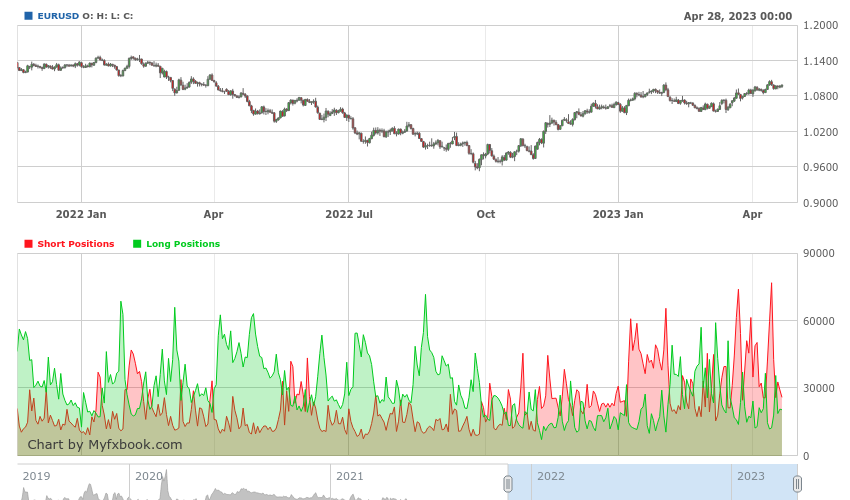
\includegraphics[scale=0.4]{p1.png}    
\end{center}